% ASSERT_CONVENTION: natural_units=natural, metric_signature=mostly_minus, fourier_convention=physics, coupling_convention=alpha_s, generator_normalization=T(fund)=1/2, covariant_derivative_sign=D_mu=partial_mu-igA
%
% Lecture 4: N=2 SUSY, the Coulomb Branch, and the Origin of Magnetic Quarks
% Part of: The Dualised Standard Model -- Part III Lecture Notes
%
% SUSY-specific conventions (continued from Lectures 2-3):
%   R-charge: R[Q] = (N_f - N_c)/N_f, R[W] = 2
%   R_fermion = R_superfield - 1 for chiral multiplet fermions
%   R_gaugino = +1 (directly; gaugino is NOT a chiral superfield component)
%   N_f counts Dirac flavour pairs
%   N=2 counting: N_f hypermultiplets = N_f pairs of N=1 chirals;
%     adjoint Phi from N=2 vector multiplet NOT counted in N_f
%   FI term: V_FI = xi D, [xi] = [mass]^2
%   Deformation: W_def = mu Tr Phi^2, [mu] = [mass]
%
\documentclass[11pt,a4paper]{article}
% ASSERT_CONVENTION: natural_units=natural, metric_signature=mostly_minus, fourier_convention=physics, coupling_convention=alpha_s, generator_normalization=T(fund)=1/2, covariant_derivative_sign=D_mu=partial_mu-igA
%
% CONVENTIONS (Seiberg hep-th/9411149)
% Metric: (+,-,-,-) (mostly minus)
% T(fund) = 1/2 per Weyl fermion
% b_0 = (11N_c - 2N_f)/3 for N_f Dirac flavours
% D_mu = partial_mu - ig A_mu^a T^a
% A(fund) = 1 (cubic anomaly coefficient per fundamental Weyl fermion)
% alpha_s = g_s^2 / (4 pi)
% R[Q] = (N_f - N_c)/N_f; R[W] = 2
% N_f counts Dirac flavour pairs (each = 2 Weyl fermions)
%
% This file is \input{} by all lecture files.

%% ---------- Document class ----------
% (loaded by the wrapper; preamble only provides packages and macros)

%% ---------- Standard packages ----------
\usepackage{amsmath,amssymb,amsthm,mathtools}
\usepackage{hyperref}
\usepackage[capitalise,noabbrev]{cleveref}
\usepackage{enumitem}
\usepackage{booktabs}
\usepackage{array}
\usepackage{xcolor}
\usepackage{tikz}
\usetikzlibrary{arrows.meta,decorations.markings,positioning,calc}
\usepackage{fancybox}
\usepackage{tcolorbox}
\tcbuselibrary{skins,breakable}
\usepackage{slashed}              % Feynman slash notation
\usepackage{cite}                 % compressed citation lists

%% ---------- Hyperref configuration ----------
\hypersetup{
  colorlinks=true,
  linkcolor=blue!70!black,
  citecolor=green!50!black,
  urlcolor=blue!80!black,
  pdfauthor={Part III Lecture Notes},
  pdftitle={The Dualised Standard Model}
}

%% ---------- Theorem environments ----------
\theoremstyle{plain}
\newtheorem{theorem}{Theorem}[section]
\newtheorem{lemma}[theorem]{Lemma}
\newtheorem{proposition}[theorem]{Proposition}
\newtheorem{corollary}[theorem]{Corollary}

\theoremstyle{definition}
\newtheorem{definition}[theorem]{Definition}
\newtheorem{example}[theorem]{Example}
\newtheorem{exercise}{Exercise}[section]

\theoremstyle{remark}
\newtheorem{remark}[theorem]{Remark}

%% ---------- Physics macros: gauge groups and representations ----------
\newcommand{\Nc}{N_{\!c}}
\newcommand{\Nf}{N_{\!f}}
\newcommand{\SU}[1]{\mathrm{SU}(#1)}
\newcommand{\UU}[1]{\mathrm{U}(#1)}

% Representations
\newcommand{\fund}{\square}
\newcommand{\antifund}{\overline{\square}}
\newcommand{\adj}{\mathrm{adj}}
\newcommand{\antisym}{\wedge^{\!2}}        % antisymmetric rank-2
\newcommand{\sym}{\mathrm{S}_2}           % symmetric rank-2

%% ---------- Physics macros: group theory constants ----------
% Dynkin index: Tr(T^a T^b) = T(R) delta^{ab}
\newcommand{\Tfund}{\tfrac{1}{2}}          % T(fund) = 1/2 per Weyl fermion
\newcommand{\Tadj}{\Nc}                    % T(adj) = N_c
\newcommand{\Cfund}{\frac{\Nc^2 - 1}{2\Nc}}  % C_2(fund)
\newcommand{\Cadj}{\Nc}                    % C_2(adj)

% Cubic anomaly coefficient: A(R) = Tr_R[T^a {T^b, T^c}] with A(fund) = 1
\newcommand{\Afund}{1}

%% ---------- Physics macros: beta function ----------
\newcommand{\bzero}{b_0}
\newcommand{\bone}{b_1}
\newcommand{\alphas}{\alpha_s}
\newcommand{\gs}{g_s}

%% ---------- Physics macros: SUSY / R-charge ----------
\newcommand{\Rcharge}[1]{R[#1]}
\newcommand{\Wsup}{W}                      % superpotential

%% ---------- Physics macros: covariant derivative and field strength ----------
\newcommand{\Dmu}{D_\mu}
\newcommand{\Fmn}{F_{\mu\nu}}
\newcommand{\Ftilde}{\widetilde{F}_{\mu\nu}}

%% ---------- Physics macros: common abbreviations ----------
\newcommand{\ie}{\textit{i.e.}}
\newcommand{\eg}{\textit{e.g.}}
\newcommand{\cf}{\textit{cf.}}
\newcommand{\IR}{\ensuremath{\mathrm{IR}}}
\newcommand{\UV}{\ensuremath{\mathrm{UV}}}
\newcommand{\AF}{\ensuremath{\mathrm{AF}}}
\newcommand{\BZ}{\ensuremath{\mathrm{BZ}}}
\newcommand{\NSVZ}{\ensuremath{\mathrm{NSVZ}}}
\newcommand{\SQCD}{\ensuremath{\mathrm{SQCD}}}
\newcommand{\QCD}{\ensuremath{\mathrm{QCD}}}
\newcommand{\SM}{\ensuremath{\mathrm{SM}}}
\newcommand{\Tr}{\mathrm{Tr}}

%% ---------- Convention box macro ----------
\newtcolorbox{conventionbox}[1][]{%
  enhanced,
  colback=blue!5!white,
  colframe=blue!60!black,
  fonttitle=\bfseries,
  title={Conventions},
  #1
}

%% ---------- Comparison table style ----------
\newtcolorbox{comparisontable}[1][]{%
  enhanced,
  colback=orange!5!white,
  colframe=orange!70!black,
  fonttitle=\bfseries,
  title={Comparison},
  #1
}

%% ---------- Warning / important box ----------
\newtcolorbox{warningbox}[1][]{%
  enhanced,
  colback=red!5!white,
  colframe=red!70!black,
  fonttitle=\bfseries,
  title={Important},
  #1
}

%% ---------- Preview / forward-reference box ----------
\newtcolorbox{previewbox}[1][]{%
  enhanced,
  colback=green!5!white,
  colframe=green!50!black,
  fonttitle=\bfseries,
  title={Preview},
  #1
}

%% ---------- Page layout ----------
\usepackage[margin=2.5cm]{geometry}
\setlength{\parskip}{0.4em}
\setlength{\parindent}{0em}

%% ---------- Section formatting ----------
\usepackage{titlesec}
\titleformat{\section}{\Large\bfseries}{\thesection}{1em}{}
\titleformat{\subsection}{\large\bfseries}{\thesubsection}{1em}{}

%% ---------- End of preamble ----------


\title{\textbf{Lecture 4: $\mathcal{N}=2$ SUSY and the Origin of Magnetic Quarks}}
\author{The Dualised Standard Model --- Part III Lecture Notes}
\date{Lent Term 2027}

\begin{document}
\maketitle

\tableofcontents
\newpage

%% ========================================================================
%%  CONVENTIONS
%% ========================================================================

\begin{conventionbox}[title={Conventions for Lecture 4}]
All conventions from Lectures~1--3 remain in force.  Additional conventions
for $\mathcal{N}=2$ theories (following Seiberg--Witten~\cite{SW1994}
and Argyres--Plesser--Seiberg~\cite{APS1996}):

\renewcommand{\arraystretch}{1.3}
\begin{tabular}{@{}l l l@{}}
\toprule
\textbf{Quantity} & \textbf{Convention} & \textbf{Comment} \\
\midrule
Units & $\hbar = c = 1$ (natural) & \\
Metric & $\eta_{\mu\nu} = \mathrm{diag}(+1,-1,-1,-1)$ & mostly minus \\
Dynkin index & $\Tr(T^a T^b) = \Tfund\, \delta^{ab}$ & $T(\fund) = \Tfund$ \\
$\Nf$ counting (${}\mathcal{N}=2$) & $\Nf$ hypermultiplets & each = $(Q_i, \widetilde{Q}_i)$ \\
Adjoint & $\Phi_{\adj}$ from $\mathcal{N}=2$ vector & NOT counted in $\Nf$ \\
FI parameter & $\xi$, \;$[\xi] = [\mathrm{mass}]^2$ & real parameter \\
Deformation & $\Wsup_{\mathrm{def}} = \mu\,\Tr\Phi^2$, \;$[\mu] = [\mathrm{mass}]$ & adjoint mass \\
Coulomb branch & parametrised by $u_k = \langle\Tr\Phi^k\rangle$ & $k = 2,\ldots,\Nc$ \\
\bottomrule
\end{tabular}
\end{conventionbox}

\begin{warningbox}[title={$\mathcal{N}=1$ / $\mathcal{N}=2$ counting}]
The decomposition of $\mathcal{N}=2$ multiplets into $\mathcal{N}=1$
components is the single most common source of counting errors
when relating $\mathcal{N}=2$ and $\mathcal{N}=1$ results.  See the
table in \S\ref{sec:multiplets} and use it every time a formula crosses
from one language to the other.
\end{warningbox}


%% ========================================================================
%%  SECTION 1: Extended SUSY -- N=2 Multiplets
%% ========================================================================
\section{Extended Supersymmetry: $\mathcal{N}=2$ Multiplets}
\label{sec:multiplets}

In Lectures~2--3 we worked with $\mathcal{N}=1$ supersymmetry: a single
supercharge $Q_\alpha$ (plus its conjugate $\bar{Q}_{\dot\alpha}$).
$\mathcal{N}=2$ supersymmetry has \emph{two} supercharges $Q_\alpha^I$,
$I = 1,2$, and its multiplets are correspondingly larger.  We shall
not develop the $\mathcal{N}=2$ superfield formalism; instead, we
decompose every $\mathcal{N}=2$ multiplet into $\mathcal{N}=1$ language,
which is sufficient for our purposes.

\subsection{The $\mathcal{N}=2$ vector multiplet}

The $\mathcal{N}=2$ vector multiplet contains, in $\mathcal{N}=1$
language:
\begin{itemize}
  \item An $\mathcal{N}=1$ \textbf{vector multiplet} $V = (A_\mu, \lambda)$,
    containing the gauge boson and one Weyl gaugino.  Both transform in the
    \textbf{adjoint} of the gauge group.
  \item An $\mathcal{N}=1$ \textbf{chiral multiplet}
    $\Phi = (\phi, \psi, F)$, also in the \textbf{adjoint}
    representation.  The scalar component $\phi$ is a complex scalar field
    valued in the Lie algebra.
\end{itemize}
The two gauginos $\lambda$ and $\psi$ are related by the second
supersymmetry.  The key point is that the adjoint chiral
$\Phi$ is \emph{part of the gauge sector}, not a matter field.

\subsection{The $\mathcal{N}=2$ hypermultiplet}

The $\mathcal{N}=2$ hypermultiplet contains, in $\mathcal{N}=1$ language:
\begin{itemize}
  \item Two $\mathcal{N}=1$ \textbf{chiral multiplets}: $Q_i$ in the
    fundamental ($\fund$) and $\widetilde{Q}_i$ in the antifundamental
    ($\antifund$) of the gauge group, for $i = 1,\ldots,\Nf$.
\end{itemize}
Each hypermultiplet contributes one unit to $\Nf$.

\subsection{Decomposition table}
\label{ssec:decomp-table}

\begin{tcolorbox}[
  enhanced,
  colback=blue!5!white,
  colframe=blue!70!black,
  fonttitle=\bfseries,
  title={$\mathcal{N}=2 \to \mathcal{N}=1$ Decomposition}
]
\renewcommand{\arraystretch}{1.5}
\begin{tabular}{@{} l l l l @{}}
\toprule
\textbf{$\mathcal{N}=2$ multiplet} & \textbf{$\mathcal{N}=1$ content}
  & \textbf{Representation} & \textbf{$\Nf$ counting} \\
\midrule
Vector multiplet & $V + \Phi_{\adj}$
  & both in $\adj$ & $\Phi_{\adj}$ \textbf{not} counted in $\Nf$ \\
Hypermultiplet & $Q_i + \widetilde{Q}_i$
  & $\fund + \antifund$ & each hyper $= 1$ unit of $\Nf$ \\
\bottomrule
\end{tabular}
\end{tcolorbox}

\subsection{$\mathcal{N}=2$ SQCD}

$\mathcal{N}=2$ SQCD with gauge group $\SU{\Nc}$ and $\Nf$
hypermultiplets is specified by:
\begin{itemize}
  \item \textbf{Gauge sector:} one $\mathcal{N}=2$ vector multiplet
    (= $V + \Phi_{\adj}$ in $\mathcal{N}=1$ language).
  \item \textbf{Matter:} $\Nf$ hypermultiplets
    (= $\Nf$ pairs $(Q_i, \widetilde{Q}_i)$ in $\mathcal{N}=1$ language).
  \item \textbf{Superpotential:} The $\mathcal{N}=2$ algebra requires
    \begin{equation}\label{eq:W-N2}
      \Wsup_{\mathcal{N}=2} = \sqrt{2}\, Q_i\, \Phi\, \widetilde{Q}^i\,,
    \end{equation}
    where $\Phi$ is the adjoint chiral from the vector multiplet.  This
    Yukawa coupling is \emph{not} a choice---it is dictated by the extended
    supersymmetry.
\end{itemize}

\subsection{The $\mathcal{N}=2$ beta function}

The one-loop beta function coefficient for $\mathcal{N}=2$ $\SU{\Nc}$
with $\Nf$ hypermultiplets is:
\begin{equation}\label{eq:b0-N2}
  \boxed{b_0^{\,\mathcal{N}=2} = 2\Nc - \Nf\,.}
\end{equation}

\textbf{Verification via $\mathcal{N}=1$ decomposition.}
In $\mathcal{N}=1$ language, the matter content of $\mathcal{N}=2$ SQCD
consists of:
\begin{itemize}
  \item $\Nf$ chiral pairs $(Q_i, \widetilde{Q}_i)$ in the fundamental
    --- contributing $\Nf$ to the $\mathcal{N}=1$ beta function.
  \item One chiral multiplet $\Phi$ in the adjoint --- contributing $\Nc$
    (since $T(\adj) = \Nc$).
\end{itemize}
The $\mathcal{N}=1$ beta function gives:
\begin{equation}\label{eq:b0-N1-check}
  b_0^{\,\mathcal{N}=1} = 3\Nc - \Nf - \Nc = 2\Nc - \Nf\,.
\end{equation}
This matches~\eqref{eq:b0-N2} exactly, as it must.
\quad$\checkmark$

\medskip

Asymptotic freedom requires $b_0^{\,\mathcal{N}=2} > 0$, \ie:
\begin{equation}\label{eq:N2-AF}
  \Nf < 2\Nc
  \qquad\text{($\mathcal{N}=2$ asymptotic freedom).}
\end{equation}

\begin{remark}[$\mathcal{N}=2$ conformal window]
  For $\Nf = 2\Nc$, the $\mathcal{N}=2$ theory is exactly conformal at
  the origin of moduli space.  For $\Nf < 2\Nc$ it is asymptotically
  free.  There is no analogue of the Seiberg conformal window in the
  $\mathcal{N}=2$ setting; the extended supersymmetry is too constraining.
\end{remark}


%% ========================================================================
%%  SECTION 2: The Coulomb Branch
%% ========================================================================
\section{The Coulomb Branch}
\label{sec:coulomb}

\subsection{Definition}

The adjoint scalar $\phi$ in the $\mathcal{N}=2$ vector multiplet can
acquire a vacuum expectation value (VEV).  Since $\phi$ transforms in the
adjoint, its VEV can be diagonalised by a gauge transformation:
\begin{equation}\label{eq:Phi-vev}
  \langle\phi\rangle = \mathrm{diag}(a_1, a_2, \ldots, a_{\Nc})\,,
  \qquad \sum_{i=1}^{\Nc} a_i = 0\,,
\end{equation}
where the tracelessness condition follows from $\SU{\Nc}$.

At a \emph{generic} point where all $a_i$ are distinct, the gauge group
is broken to its maximal abelian subgroup:
\begin{equation}\label{eq:coulomb-breaking}
  \SU{\Nc} \;\longrightarrow\; \UU{1}^{\Nc - 1}\,.
\end{equation}
The low-energy theory is a collection of $(\Nc - 1)$ abelian
$\mathcal{N}=2$ gauge multiplets --- a free $\UU{1}^{\Nc-1}$ gauge
theory.  This is an abelian \textbf{Coulomb phase}, hence the name.

\subsection{Gauge-invariant coordinates}

The moduli space of vacua is parametrised by gauge-invariant quantities:
\begin{equation}\label{eq:uk}
  u_k = \langle\Tr\phi^k\rangle\,,
  \qquad k = 2, 3, \ldots, \Nc\,.
\end{equation}
For $\SU{2}$, there is a single complex parameter:
\begin{equation}\label{eq:u-SU2}
  u = \langle\Tr\phi^2\rangle = a_1^2 + a_2^2 = 2a^2\,,
\end{equation}
where $a_1 = -a_2 = a$ (tracelessness).  The Coulomb branch is a complex
plane parametrised by $u$.

\subsection{Classical singularities}

Classically, the Coulomb branch is smooth except at the \textbf{origin}
$u = 0$ (equivalently $a = 0$), where the gauge symmetry is enhanced
back to $\SU{2}$ and the $W$-bosons become massless.

Quantum mechanically, the story changes dramatically.


%% ========================================================================
%%  SECTION 3: Seiberg-Witten Solution -- Executive Summary
%% ========================================================================
\section{The Seiberg--Witten Solution: Executive Summary}
\label{sec:SW}

\begin{warningbox}[title={Scope of this section}]
  We \textbf{state} the key results of the Seiberg--Witten solution
  without derivation.  The full derivation --- involving an auxiliary
  elliptic curve, its periods, monodromies, and the instanton expansion
  --- would require several additional lectures.  We refer
  to~\cite{SW1994,SW1994b} for the original papers
  and to Alvarez-Gaum\'e and Hassan~\cite{AGH1997} for a pedagogical
  treatment.
\end{warningbox}

\subsection{The exact prepotential}

Seiberg and Witten~\cite{SW1994} showed that the \emph{exact} low-energy
effective action of $\mathcal{N}=2$ $\SU{2}$ pure gauge theory is
determined by a holomorphic function $\mathcal{F}(a)$, the
\textbf{prepotential}, which encodes all couplings and interactions
of the $\UU{1}$ theory on the Coulomb branch.  The key constraint is
that $\mathcal{F}$ must be consistent with the global structure of the
moduli space, including its singularities and monodromies.

The solution is encoded in an auxiliary \textbf{elliptic curve} (the
Seiberg--Witten curve), whose periods determine $a$ and $a_D = \partial
\mathcal{F}/\partial a$ as functions of $u$.  We state the result without
deriving it.

\subsection{Singular points of the Coulomb branch}

The central result of~\cite{SW1994} is:

\begin{tcolorbox}[
  enhanced,
  colback=blue!5!white,
  colframe=blue!70!black,
  fonttitle=\bfseries\large,
  title={Seiberg--Witten Solution for $\SU{2}$},
  breakable
]
The quantum Coulomb branch of $\mathcal{N}=2$ $\SU{2}$ pure gauge theory
has \textbf{two} singular points:
\begin{enumerate}
  \item At $u = +\Lambda_{\mathcal{N}=2}^2$: a magnetic \textbf{monopole}
    (with charges $(n_e, n_m) = (0, 1)$) becomes massless.
  \item At $u = -\Lambda_{\mathcal{N}=2}^2$: a \textbf{dyon}
    (with charges $(n_e, n_m) = (1, 1)$) becomes massless.
\end{enumerate}
Here $\Lambda_{\mathcal{N}=2}$ is the dynamical scale of the
$\mathcal{N}=2$ theory.  The classical singularity at $u = 0$ (massless
$W$-bosons) is \textbf{split} into two singularities by quantum effects.
At each singular point, the low-energy theory is a $\UU{1}$ gauge theory
coupled to the massless monopole or dyon.
\end{tcolorbox}

\subsection{Physical picture}

\begin{figure}[ht]
\centering
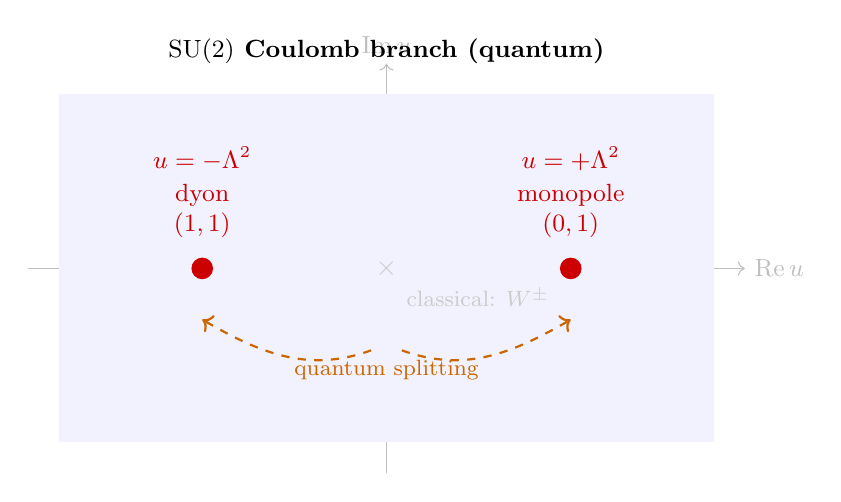
\begin{tikzpicture}[scale=1.3]
  % Axes
  \draw[->,gray!50] (-3.5,0) -- (3.5,0) node[right,gray!50] {\small $\mathrm{Re}\,u$};
  \draw[->,gray!50] (0,-2) -- (0,2) node[above,gray!50] {\small $\mathrm{Im}\,u$};

  % Coulomb branch (shaded region)
  \fill[blue!5] (-3.2,-1.7) rectangle (3.2,1.7);

  % Classical singularity (crossed out)
  \node[gray!40] at (0,0) {$\times$};
  \node[below right,gray!40,font=\footnotesize] at (0.1,-0.1)
    {classical: $W^{\pm}$};

  % Quantum singular points
  \fill[red!80!black] (-1.8,0) circle (3pt);
  \fill[red!80!black] (1.8,0) circle (3pt);

  % Labels
  \node[above,red!80!black,font=\small,align=center] at (1.8,0.2)
    {$u = +\Lambda^2$\\[1pt]monopole\\$(0,1)$};
  \node[above,red!80!black,font=\small,align=center] at (-1.8,0.2)
    {$u = -\Lambda^2$\\[1pt]dyon\\$(1,1)$};

  % Arrow showing quantum splitting
  \draw[->,thick,dashed,orange!80!black]
    (-0.15,-0.8) to[out=200,in=-30] (-1.8,-0.5);
  \draw[->,thick,dashed,orange!80!black]
    (0.15,-0.8) to[out=-20,in=210] (1.8,-0.5);
  \node[below,orange!80!black,font=\footnotesize] at (0,-0.8)
    {quantum splitting};

  % Title
  \node[above,font=\bfseries\small] at (0,1.9)
    {$\SU{2}$ Coulomb branch (quantum)};
\end{tikzpicture}
\caption{The Coulomb branch of $\mathcal{N}=2$ $\SU{2}$ pure gauge
theory.  Classically, there is a single singularity at $u = 0$ where
$W$-bosons become massless.  Quantum mechanically, this splits into two
singularities at $u = \pm\Lambda^2$, where a monopole and a dyon
(respectively) become massless.}
\label{fig:coulomb-branch}
\end{figure}

The physical picture is remarkable: the theory dynamically generates new
light states --- monopoles and dyons --- that are \emph{not} present in
the perturbative spectrum.  These are solitonic states whose mass is
determined by the BPS formula:
\begin{equation}\label{eq:BPS}
  M = \sqrt{2}\,|n_e\, a + n_m\, a_D|\,,
\end{equation}
where $(n_e, n_m)$ are the electric and magnetic charges, and $a$, $a_D$
are the special coordinates on the Coulomb branch.  At the singular
points, $a_D \to 0$ (monopole point) or $a - a_D \to 0$ (dyon point),
making the corresponding state massless.

\subsection{$\SU{\Nc}$ with $\Nf$ hypermultiplets}

For $\SU{\Nc}$ with $\Nf$ hypermultiplets (Seiberg--Witten
II~\cite{SW1994b}), the Coulomb branch has a richer structure:
\begin{itemize}
  \item The moduli space is $(\Nc - 1)$-dimensional, parametrised by
    $u_2, \ldots, u_{\Nc}$.
  \item There are multiple singular loci where different magnetic and
    dyonic states become massless.
  \item The monopoles carry \textbf{flavour quantum numbers} because the
    BPS mass formula~\eqref{eq:BPS} involves the quark masses
    (which enter through the hypermultiplet VEVs), and the monopole
    wavefunctions ``feel'' the flavour structure of the quarks via
    their fermionic zero modes.
\end{itemize}

The last point is crucial: the monopoles are not flavour-singlets.  They
transform non-trivially under the global flavour symmetry
$\SU{\Nf}_L \times \SU{\Nf}_R$.


%% ========================================================================
%%  SECTION 4: The Fayet-Iliopoulos Mechanism
%% ========================================================================
\section{The Fayet--Iliopoulos Mechanism}
\label{sec:FI}

Before presenting the deformation argument, we need one more ingredient:
the Fayet--Iliopoulos (FI) $D$-term~\cite{FI1974}.

\subsection{Definition}

For a $\UU{1}$ gauge factor, there is a unique gauge-invariant and
supersymmetric term that can be added to the Lagrangian:
\begin{equation}\label{eq:FI}
  \boxed{\mathcal{L}_{\mathrm{FI}} = \xi\, D\,,}
\end{equation}
where $D$ is the auxiliary field of the $\UU{1}$ vector multiplet and
$\xi$ is a real parameter.

\textbf{Dimensional analysis:} $[D] = [\mathrm{mass}]^2$ (since $D$ is
an auxiliary field with no kinetic term, and $[\mathcal{L}] =
[\mathrm{mass}]^4$), therefore:
\begin{equation}\label{eq:xi-dim}
  [\xi] = [\mathrm{mass}]^2\,.
\end{equation}

\subsection{Effect on the D-term potential}

In the presence of the FI term, the $D$-term scalar potential becomes:
\begin{equation}\label{eq:VD-FI}
  V_D = \frac{1}{2}\left(g\sum_i q_i\,|\phi_i|^2 + \xi\right)^{\!2},
\end{equation}
where $q_i$ are the $\UU{1}$ charges of the scalar fields $\phi_i$.

If $\xi \neq 0$, the minimum of $V_D$ requires
$g\sum_i q_i\,|\phi_i|^2 = -\xi$, which forces at least one scalar
$\phi_i$ to acquire a non-zero VEV.  This breaks the $\UU{1}$ gauge
symmetry.

\subsection{Application to the Coulomb branch}

On the Coulomb branch of $\mathcal{N}=2$ theories, the unbroken gauge
group is $\UU{1}^{\Nc-1}$.  Each $\UU{1}$ factor can, in principle,
have an FI parameter.  When the adjoint mass deformation
(Section~\ref{sec:APS}) lifts the Coulomb branch, the effective FI
parameters at the surviving singular points can force the massless
monopoles to \emph{condense} (acquire VEVs).  Monopole condensation is
the dual mechanism to the Higgs effect: it produces
\textbf{confinement} of the original electric charges, by the dual
Meissner effect.
The FI $D$-term is an effective low-energy statement; its UV status depends on the embedding and may require completion at higher scales.


%% ========================================================================
%%  SECTION 5: The APS Deformation -- From N=2 to N=1
%% ========================================================================
\section{The APS Deformation: From $\mathcal{N}=2$ to $\mathcal{N}=1$}
\label{sec:APS}

We now move from the exact Seiberg--Witten analysis to the Argyres--Plesser--Seiberg \emph{interpretation} of the singularity structure.

We now present the central argument of this lecture: the identification
of the magnetic quarks of $\mathcal{N}=1$ Seiberg duality with the
monopoles and dyons of the $\mathcal{N}=2$ Coulomb
branch~\cite{APS1996}.

\subsection{The deformation}

Consider $\mathcal{N}=2$ $\SU{\Nc}$ SQCD with $\Nf$ hypermultiplets.
Add a superpotential deformation:
\begin{equation}\label{eq:W-def}
  \Wsup_{\mathrm{def}} = \mu\,\Tr\Phi^2\,,
\end{equation}
where $\Phi$ is the adjoint chiral from the $\mathcal{N}=2$ vector
multiplet and $\mu$ is a mass parameter with $[\mu] = [\mathrm{mass}]$.

\textbf{Dimensional check:} $[\Wsup] = [\mathrm{mass}]^3$, $[\Phi] =
[\mathrm{mass}]$, $[\Tr\Phi^2] = [\mathrm{mass}]^2$, so
$[\mu\,\Tr\Phi^2] = [\mathrm{mass}]^3$.
\quad$\checkmark$

This deformation breaks $\mathcal{N}=2 \to \mathcal{N}=1$: the
$\mathcal{N}=2$ superpotential~\eqref{eq:W-N2} plus the mass
term~\eqref{eq:W-def} is not compatible with the second supercharge.
The total $\mathcal{N}=1$ superpotential is:
\begin{equation}\label{eq:W-total}
  \Wsup = \sqrt{2}\, Q\Phi\widetilde{Q} + \mu\,\Tr\Phi^2\,.
\end{equation}

\subsection{The four-step argument}

The logic of the APS argument~\cite{APS1996} proceeds in four steps:

\begin{tcolorbox}[
  enhanced,
  colback=green!5!white,
  colframe=green!60!black,
  fonttitle=\bfseries,
  title={The APS Deformation Argument}
]
\begin{enumerate}[label=\textbf{Step \arabic*.},leftmargin=*]
  \item \textbf{Start with $\mathcal{N}=2$.}  Consider $\SU{\Nc}$
    $\mathcal{N}=2$ SQCD with $\Nf$ hypermultiplets.  The theory has a
    Coulomb branch with known singularities where monopoles and dyons
    become massless.

  \item \textbf{Turn on the deformation.}  Add
    $\Wsup_{\mathrm{def}} = \mu\,\Tr\Phi^2$.  For small $\mu$, this is
    a soft perturbation of the $\mathcal{N}=2$ theory.  It generates a
    potential on the Coulomb branch:
    \[
      V \supset |\mu|^2\,|\Tr\phi^2|^2 + \cdots
    \]
    The Coulomb branch is \textbf{lifted}: the flat directions are no
    longer flat, and the theory is driven to specific minima.

  \item \textbf{Identify the vacua.}  The vacua of the deformed theory
    are located at the \textbf{singular points} of the Coulomb branch
    --- precisely the points where monopoles and dyons become massless.
    At these points, the monopoles condense (via the FI mechanism of
    \S\ref{sec:FI}), breaking the residual $\UU{1}$ gauge symmetries
    and producing a confining vacuum.

  \item \textbf{Take $\mu \to \infty$.}  As the adjoint mass $\mu$
    becomes large, the adjoint chiral $\Phi$ decouples from the
    low-energy theory.  Below the scale $\mu$, the $\mathcal{N}=1$
    field content is:
    \begin{itemize}
      \item \textbf{Gauge group:} $\SU{\Nc}$.
      \item \textbf{Matter:} $\Nf$ pairs $(Q_i, \widetilde{Q}_i)$ in the
        fundamental and antifundamental.
      \item \textbf{Superpotential:} $\Wsup = 0$ (the Yukawa coupling
        $Q\Phi\widetilde{Q}$ decouples with $\Phi$).
    \end{itemize}
    This is precisely the \textbf{electric theory} of $\mathcal{N}=1$
    Seiberg duality from Lecture~3!
\end{enumerate}
\end{tcolorbox}

\subsection{The punchline: monopoles become magnetic quarks}

The conclusion of the four-step argument is:

\begin{tcolorbox}[
  enhanced,
  colback=yellow!8!white,
  colframe=yellow!60!black,
  fonttitle=\bfseries\large,
  title={Origin of Magnetic Quarks}
]
The magnetic quarks $q_i$, $\widetilde{q}^{\,j}$ of the $\mathcal{N}=1$
Seiberg dual are identified with the \textbf{monopoles and dyons} that
become massless on the Coulomb branch of the parent $\mathcal{N}=2$
theory.  Seiberg duality for $\mathcal{N}=1$ SQCD can be understood as
a \emph{consequence} of the exact $\mathcal{N}=2$
results~\cite{APS1996}.
\end{tcolorbox}

\medskip

More specifically:
\begin{enumerate}[label=(\alph*)]
  \item The magnetic quarks are 't~Hooft--Polyakov monopoles of the
    $\SU{\Nc}$ theory, made light by the dynamics on the
    $\mathcal{N}=2$ Coulomb branch.
  \item They carry flavour quantum numbers because the monopole
    wavefunctions have fermionic zero modes from the hypermultiplet
    quarks (see \S\ref{sec:SW}, final paragraph).
  \item The magnetic gauge group $\SU{\Nf - \Nc}$ arises from the
    pattern of monopole condensation at the singular loci.
  \item The meson field $M^i{}_j$ of the magnetic theory arises from the
    adjoint scalar $\Phi$: as $\mu \to \infty$, the massive components
    of $\Phi$ decouple, but the composite operator
    $Q_i\,\Phi\,\widetilde{Q}^j$ survives as the elementary
    meson~$M^i{}_j$ in the low-energy magnetic description.
\end{enumerate}

\begin{remark}[Continuity of the vacuum]
  The argument relies on the fact that the vacuum structure varies
  \emph{continuously} as $\mu$ is increased from $0$ (pure
  $\mathcal{N}=2$) to $\infty$ (pure $\mathcal{N}=1$).  This is
  guaranteed by holomorphy of the superpotential: there are no phase
  transitions as a function of $\mu$, so the identification of
  low-energy degrees of freedom at small $\mu$ (monopoles) persists
  to large $\mu$ (magnetic quarks).
\end{remark}


%% ========================================================================
%%  SECTION 6: Summary and Physical Picture
%% ========================================================================
\section{Summary and Physical Picture}
\label{sec:summary}

\begin{tcolorbox}[
  enhanced,
  colback=green!5!white,
  colframe=green!60!black,
  fonttitle=\bfseries,
  title={Lecture 4: Summary}
]
\begin{enumerate}
  \item $\mathcal{N}=2$ SQCD has a \textbf{Coulomb branch}
    parametrised by $u_k = \langle\Tr\Phi^k\rangle$, where the gauge
    group $\SU{\Nc}$ is broken to $\UU{1}^{\Nc-1}$.

  \item The \textbf{Seiberg--Witten solution} (stated, not derived)
    shows that the quantum Coulomb branch has singular points where
    \textbf{monopoles} and \textbf{dyons} become massless.

  \item The \textbf{Fayet--Iliopoulos mechanism} ($V_{\mathrm{FI}} =
    \xi D$, $[\xi] = [\mathrm{mass}]^2$) provides a mechanism for
    monopole condensation on the Coulomb branch.

  \item The \textbf{APS deformation} $\Wsup = \mu\,\Tr\Phi^2$ breaks
    $\mathcal{N}=2 \to \mathcal{N}=1$ and drives the theory to the
    Coulomb branch singularities.

  \item As $\mu \to \infty$, the adjoint $\Phi$ decouples, recovering
    $\mathcal{N}=1$ SQCD.  The massless \textbf{monopoles} and
    \textbf{dyons} of the $\mathcal{N}=2$ theory become the
    \textbf{magnetic quarks} of $\mathcal{N}=1$ Seiberg duality.

  \item This explains \emph{where} the magnetic degrees of freedom come
    from and \emph{why} they carry flavour quantum numbers.
\end{enumerate}
\end{tcolorbox}

\begin{previewbox}[title={Preview: Lectures 5--6}]
  In non-supersymmetric theories, we do not have the $\mathcal{N}=2$
  derivation.  We cannot track the fate of monopoles as a function of a
  continuously tuneable parameter.  Instead, we must rely on
  \textbf{anomaly matching} --- verified in Lecture~3 --- as the primary
  evidence for duality.  This is why the SUSY case is foundational: it
  provides a microscopic \emph{proof of concept} for electric--magnetic
  duality, which we then \emph{conjecture} to extend beyond the SUSY
  setting.  In Lectures~5--6, we will apply this duality framework to
  the Standard Model.
\end{previewbox}


%% ========================================================================
%%  BIBLIOGRAPHY
%% ========================================================================
\begin{thebibliography}{99}

\bibitem{SW1994}
  N.~Seiberg and E.~Witten,
  ``Electric--magnetic duality, monopole condensation, and confinement
  in $\mathcal{N}=2$ supersymmetric Yang--Mills theory,''
  \textit{Nucl.~Phys.} \textbf{B426} (1994) 19;
  \textit{Erratum:} \textbf{B430} (1994) 485
  [\texttt{hep-th/9407087}].

\bibitem{SW1994b}
  N.~Seiberg and E.~Witten,
  ``Monopoles, duality and chiral symmetry breaking
  in $\mathcal{N}=2$ supersymmetric QCD,''
  \textit{Nucl.~Phys.} \textbf{B431} (1994) 484
  [\texttt{hep-th/9408099}].

\bibitem{APS1996}
  P.~C.~Argyres, M.~R.~Plesser, and N.~Seiberg,
  ``The moduli space of vacua of $\mathcal{N}=2$ SUSY QCD and duality
  in $\mathcal{N}=1$ SUSY QCD,''
  \textit{Nucl.~Phys.} \textbf{B471} (1996) 159
  [\texttt{hep-th/9603042}].

\bibitem{FI1974}
  P.~Fayet and J.~Iliopoulos,
  ``Spontaneously broken supergauge symmetries and Goldstone spinors,''
  \textit{Phys.~Lett.} \textbf{B51} (1974) 461.

\bibitem{AGH1997}
  L.~Alvarez-Gaum\'e and S.~F.~Hassan,
  ``Introduction to S-duality in $\mathcal{N}=2$ supersymmetric gauge
  theories (a pedagogical review of the work of Seiberg and Witten),''
  \textit{Fortsch.~Phys.} \textbf{45} (1997) 159
  [\texttt{hep-th/9701069}].

\bibitem{Seiberg1995}
  N.~Seiberg,
  ``Electric--magnetic duality in supersymmetric non-Abelian gauge
  theories,''
  \textit{Nucl.~Phys.} \textbf{B435} (1995) 129
  [\texttt{hep-th/9411149}].

\bibitem{IS1995}
  K.~Intriligator and N.~Seiberg,
  ``Lectures on supersymmetric gauge theories and electric-magnetic
  duality,''
  \textit{Nucl.~Phys.~Proc.~Suppl.} \textbf{45BC} (1996) 1
  [\texttt{hep-th/9509066}].

\bibitem{Sannino2024}
  F.~Sannino \textit{et al.},
  ``The Dualised Standard Model,''
  [\texttt{arXiv:2407.17281}].

\end{thebibliography}

\end{document}
